\documentclass[12pt]{article}

\usepackage[utf8]{inputenc}
\usepackage[brazil]{babel}
\usepackage{amsmath,amssymb}
\usepackage{pdfsync}
\usepackage[all]{xy}
\usepackage{color}
\usepackage{graphicx}
\usepackage[]{algorithm2e}

\newcommand{\resposta}[1]{ \noindent {\bf Solução}.{\color{blue} #1}}

\title{{\large Universidade de Brasília \\ Instituto de Ciências Exatas \\
Departamento de Ciência da Computação} \\[1cm]
CIC 117536 - Projeto e Análise de Algoritmos \\[.5cm]  Terceira Prova \\[.5cm] Turma: B}
\author{{\bf NP-completude}}
\date{Prof. Flávio L. C. de Moura \\[.5cm] \today}

\begin{document}
\maketitle

\begin{enumerate}
\item {\bf (2.5 pontos)} O problema 2-SAT tem como instâncias as
  fórmulas lógicas formadas por conjunções de disjunções de até dois
  literais, onde um literal é uma variável booleana ou a negação de
  uma variável booleana. Por exemplo, a expressão a seguir é uma
  instância de 2-SAT:

  $$(x_1\lor \neg x_2)\land (\neg x_1 \lor \neg x_3) \land (x_1 \lor x_2) \land x_3$$

  Prove que 2-SAT $\in$ P.

 
 \resposta{
    O problema 2-SAT pode ser resolvido em tempo polinomial fazendo uma transformação da fórmula original para um grafo. Primeiramente é possível observar que uma clausula
    qualquer \(A \lor B\) é equivalente a \(\neg A \implies B\) assim como \(\neg B \implies A\) o que significa dizer que ~A verdadeiro implica em B ser verdadeiro para satisfazer a cláusula. Logo podemos
    construir uma grafo onde cada cláusula do 2-SAT irá adicionar 2 arestas, e cada variável A irá acrescentar 2 vértices \(\neg A\) e A no grafo, o que pode ser feito em tempo polinomial relativo a representação na entrada. Sabendo da construção acima, é possivel mostrar por contradição que caso exista um caminho de uma variável X para \(\neg X\) e um caminho de \(\neg X\) para X então a fórmula não será satisfazivel.

\\ Prova:
	Suponha que existe um caminho X para \(\neg X\) e \(\neg X\) para X no grafo e também uma designação de valores para vada variável da fórmula original para a qual está será verdadeira. Suponha que existe o seguinte caminho:
			
\[X \implies ... \implies A \implies B \implies ... \implies \neg X\]
		
    Sabendo que X é verdadeiro neste caminho entao \(\neg X\) deverá ser falso portando todas as variáveis no intervalo [B,\(\neg X\)] devem ser falsas para que estas clausulas possam ser verdadeiras,da mesma forma para o caminho [X, A] todas as variaveis devem ser verdadeiras para que estas cláusulas também sejam verdadeiras. Porém existe um impasse na cláusula \(A \implies B\) onde B deverá ser falso e A deverá ser verdadeiro o que gera um valor verdade falso para esta cláusula fazendo com que a fórmula não seja satisfazivel para X = v. O mesmo raciocinio pode ser feito para o caminho \(\neg X \implies X\) que implicaria na fórmula original também não ser satisfazivel para um valor de \(\neg X\) = v. Portanto se existem estes dois caminhos não é possivel encontrar um valor verdade para X que satisfaça a fórmula orignal o que contradiz a hipótese de que tal designação existe. Para encontrar um tal caminho é possivel rodar um algortimo de componentes fortemente conexas O(V+E) e verificar se em alguma componente X e \(\neg X\), para alguma variável da fórmula, aparecem.
    
 }
  
\item {\bf (2.5 pontos)} Em aula, assumimos que SAT é um problema
  NP-completo (Teorema de Cook-Levin), e a partir deste fato mostramos
  que 3-SAT e CLIQUE também são problemas NP-completos. As reduções
  foram feitas de acordo com o seguinte diagrama:

  $$\xymatrix{
    SAT \ar[d] \\
    3\mbox{-}SAT \ar[d] \\
    CLIQUE 
  }$$
  
  Um ciclo Hamiltoniano é um ciclo simple que visita cada vértice de
  um grafo exatamente uma vez. Considere o problema de decisão
  HAM-CYCLE que pergunta se um dado grafo (não-dirigido) $G$ possui um
  ciclo Hamiltoniano. Mostre que HAM-CYCLE é um problema
  NP-completo. Sua solução deve ser construída a partir de SAT, 3-SAT
  ou CLIQUE. Caso, você não veja como reduzir diretamente HAM-CYCLE a
  partir destes, mas sabe como fazê-lo a partir de um certo problema
  $Q$ então inicialmente mostre que $Q$ é NP-completo a partir de SAT,
  3-SAT ou CLIQUE, e assim por diante. Digamos que você não saiba como
  mostrar que $Q$ é NP-completo diretamente a partir de SAT, 3-SAT ou
  CLIQUE, mas você sabe como fazê-lo a partir de outro problema $Q'$,
  e também sabe como mostrar que $Q'$ é NP-completo a partir de 3-SAT,
  por exemplo. Então o diagrama correspondente à sua solução seria:

$$\xymatrix{
  SAT \ar[d] & & & \\
  3\mbox{-}SAT \ar[d]\ar[r] & Q' \ar[r] & Q \ar[r] & \mbox{HAM-CYCLE}  \\
  CLIQUE & & & 
}$$

E todas as reduções (de 3-SAT para $Q'$, de $Q'$ para $Q$ e de $Q$ para HAM-CYCLE) devem ser detalhadas na sua solução.

\resposta{
    
    Para provar que HAM-CYCLE é NP-completo precisamos provar duas coisas:
    
    Que é possível conferir que um certo caminho P = (v1,v2,...,vn ), vn = v1,  forma um caminho hamiltoniano em um grafo G = (V,E) em tempo polinomial, assim provando que HAM-CYCLE está em NP.
    E que é possível reduzir HAM-CYCLE a partir de um problema NP-completo em tempo polinomial, provando que é NP-Difícil.
    
    Para resolver o primeiro ponto, basta percorrer o caminho, conferindo que existe uma aresta conectando todos os pares de vértices consecutivos, que cada vértice aparece apenas uma vez, exceto o primeiro e o último que devem ser iguais, e que todos os vértices de V estão em P. Esse percorrimento ocorre em tempo polinomial.
    
    Para resolver o segundo ponto, provaremos que  \(3SAT \leq p HAMCYCLE\)
    
    Nós representamos cada variável Xi em uma fórmula lógica como uma estrutura em diamante, como representado na figura 1, e adicionamos um vértice para cada cláusula conjuntiva.
    
\begin{figure}[ht]
\centering
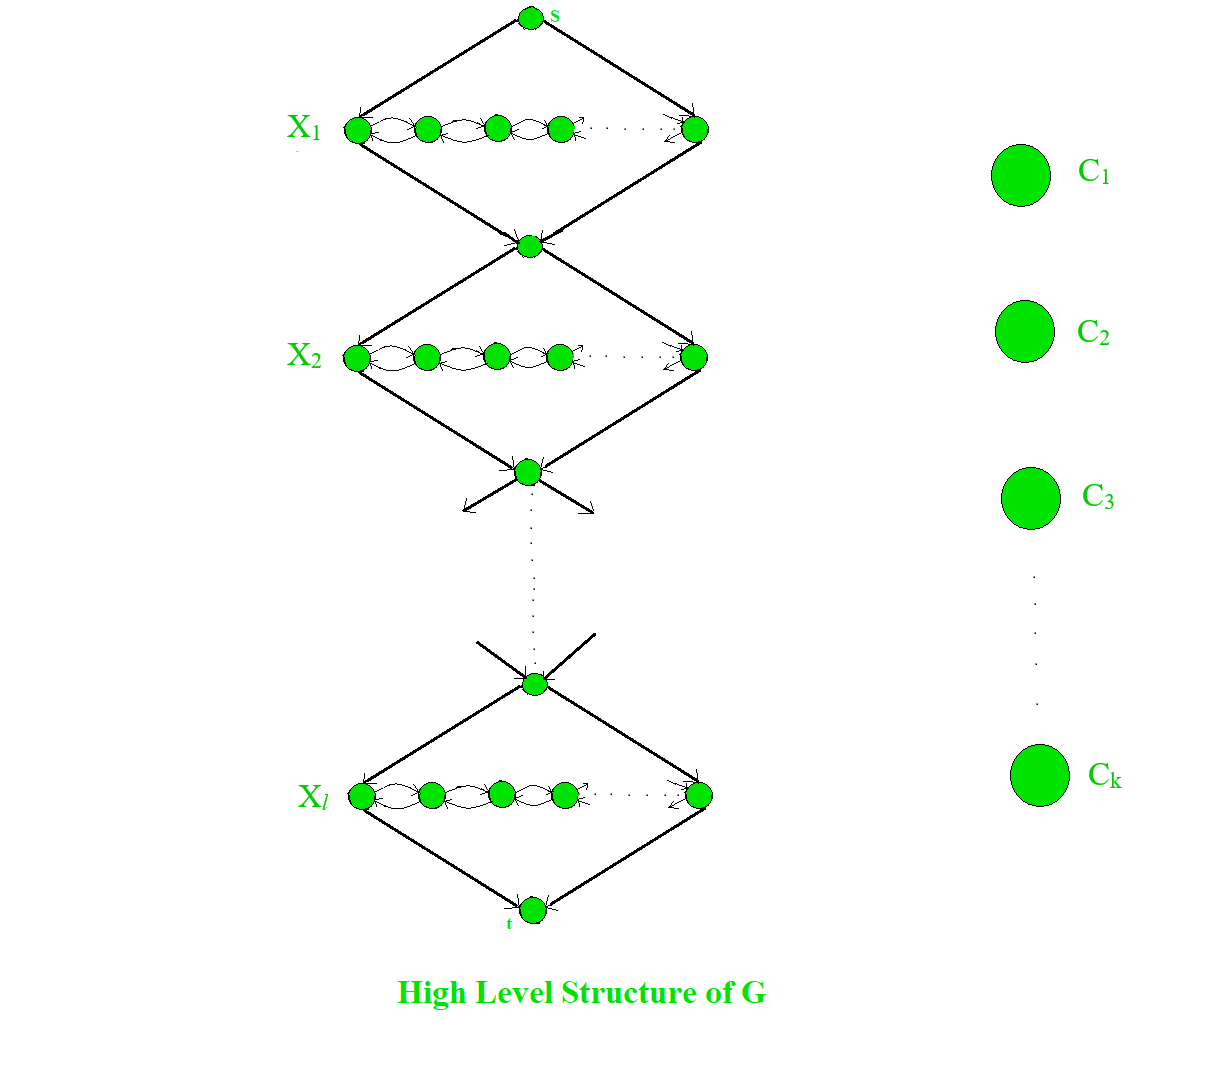
\includegraphics[width=.9\textwidth]{Estrutura de diamantes.png}
\caption{Estrutura de diamantes}
\label{fig:}
\end{figure}
    
    Cada diamante contem um fileira de 2k vértices, sendo k o número de cláusulas, mais k-1 vértices entre cada par de vértices. Com os dois vértices pertencentes ao diamante, temos um total de 3k+1 vértices, como está representado na figura 2.
    
\begin{figure}[ht]
\centering
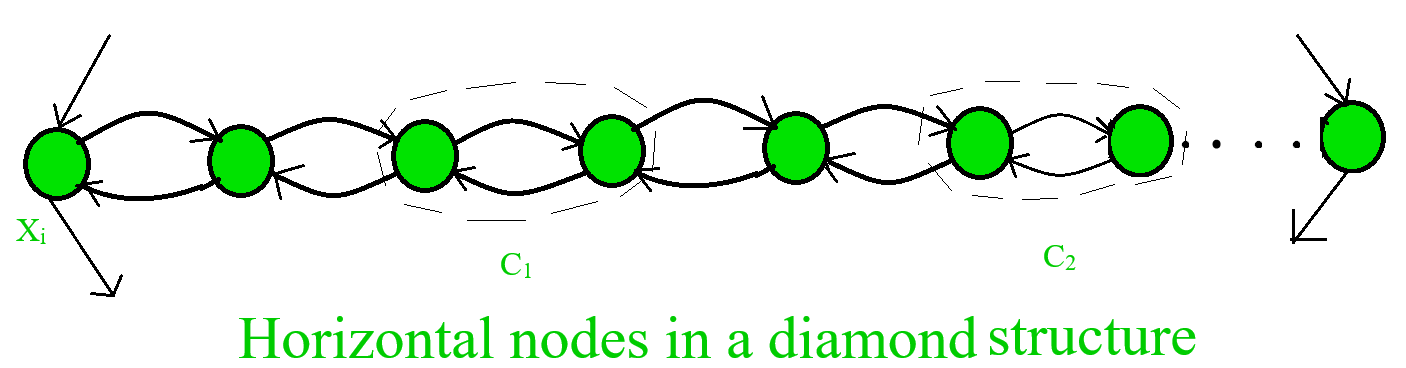
\includegraphics[width=.9\textwidth]{Fileiras no diamante.png}
\caption{Fileiras no diamante}
\label{fig:}
\end{figure}
    
    Para cada variável Xi que aparece em uma cláusula j, conectamos o par de vértices relativos a j dentro do diamante de Xi ao vértice Cj de j, essa conexão é feita por meio de duas arestas novas inseridas no grafo, uma saíndo do vértice a esquerda do par para o vértice Cj e outra saindo de Cj para o vértice a direita do par.
    
    Para cada variável \(\neg Xi\) que aparece em uma cláusula j, conectamos o par de vértices relativos a j dentro do diamante de Xi ao vértice Cj de j, essa conexão é feita por meio de duas arestas novas inseridas no grafo, uma saíndo do vértice a direita do par para o vértice Cj e outra saindo de Cj para o vértice a esquerda do par.
    
    A seguir, provaremos que se um procedimento que afirma se existe um ciclo hamiltoniano em grafos for executado sobre essa estrutura, ele afirmará que possui, caso a fórmula seja satisfazível, e que não possui o ciclo, caso não seja.
    
    Para que o ciclo seja hamiltoniano, todos os vértices do grafo devem fazer parte do ciclo, mas para que os vértices Cj que representam cada cláusula sejam visitados, deve-se usar as arestas vindas dos diamantes que representam seus literais. Porém, caso o diamante de um certo literal Xi esteja sendo percorrido da direita para esquerda, apenas os vértices das cláusulas em que \(\neg Xi\) apareça poderão ser visitados. Caso ele esteja sendo percorrido da esquerda para direita, apenas os vértices das cláusulas em que Xi apareça poderão ser visitados.
    
    Portanto, ao se percorrer um diamante Xi, deve-se escolher um lado para percorrê-lo, caso seja percorrido da direita para a esquerda, seria como se o valor de Xi fosse falso, e todas as cláusulas em que \(\neg Xi\) aparece serão marcadas e nenhuma cláusula em que Xi aparece seriam marcadas. Caso seja percorrido da esquerda para direita, seria como se o valor de Xi fosse verdadeira, e todas as cláusulas em que Xi aparece serão marcadas e nenhuma cláusula em que \(\neg Xi\) aparece seriam marcadas.
    
    Dessa forma, para que um vértice Cj que represente uma cláusula j seja visitado, algum dos literais dentro dela tem que possuir um valor verdadeiro. Ou seja, caso o circulo hamiltoniano exista, todos os Cj foram visitados e isso resulta que todos eles possuem pelo menos um literal que possa verdadeiro, caso não exista, alguma das cláusulas não possui um literal verdadeiro sem que falseie outra cláusula.
    
}
  
\item {\bf (2.5 pontos)} Considere o seguinte jogo em um grafo
  (não-dirigido) $G$, que inicialmente contém 0 ou mais bolas de gude
  em seus vértices: um movimento deste jogo consiste em remover duas
  bolas de gude de um vértice $v\in G$, e adicionar uma bola a algum
  vértice adjacente de $v$. Agora, considere o seguinte problema: Dado
  um grafo $G$, e uma função $p(v)$ que retorna o número de bolas de
  gude no vértice $v$, existe uma sequência de movimentos que remove
  todas as bolas de $G$, exceto uma? Mostre que este problema é
  NP-completo. A mesma observação feita no exercício anterior vale
  aqui: a prova deve ser feita a partir de problemas que provamos
  serem NP-completos, e reduções intermediárias, caso existam, devem
  ser incluídas na solução.

  \resposta{
    Para provar que esse problema é NP-completo, primeiro precisamos mostrar que ele é NP, para isso temos que provar que dada uma suposta resposta para um problema, é possível verificar se ela é realmente valida ou não em tempo polinomial.
    
    Para isso supomos que existe uma sequência de movimentos sobre pares de vértices $R$ = (($V1$,$V2$),($V3$,$V4$), ... , ($Vn-1$,$Vn$)), sendo que cada movimento seria remover duas bolas do vértice a direita e adicionar uma bola ao vértice a esquerda. 
    
    Para conferir se $R$ é uma solução para um grafo $G$ = ($V$, $E$) qualquer e dada a função $p(v)$ que retorna o número de bolas de gude no vértice $v$, usamos o algoritmo 1 abaixo
    
\begin{algorithm}[H]
\KwData{sequência $R$, grafo $G$ e função $p$}
\KwResult{Se $R$ resolve o problema em questão}

\For{cada par $($u$,$v$) \in R$}{

\eIf{$($u$,$v$) \in E$ and $p(u)$ \geq 2}{
$p(u) \leftarrow p(u)-2$

$p(v) \leftarrow p(v)+1$
}{
return FALSE
}
}

$S \leftarrow FALSE$ 

\For{cada vértice $v$ \in $E$}{

\eIf{$p(u)$ $=$ 1}{
\eIf{$S$ $=$ TRUE}{
return FALSE
}{
$S \leftarrow TRUE$ 
}
}{
\eIf{$p(u)$ \neq 0}{
return FALSE
}
}
}
return S
\BlankLine

\caption{verificar uma solução para o problema das bolas}
\end{algorithm}
}

Como o algoritmo 1 executa em tempo polinomial, então é possível verificar o problema das bolas em tempo polinomial.
  
\item {\bf (2.5 pontos)} Uma fórmula booleana em {\it forma normal conjuntiva com disjunção exclusiva (FNCX)} é uma conjunção de diversas cláusulas, e cada cláusula é uma disjunção exclusiva (XOR) de diversos literais. Lembre-se que a disjunção exclusiva é dada por:

  $$\begin{array}{|l|l|l|}\hline
      a & b & a \oplus b \\ \hline
      V & V & F \\ \hline
      V & F & V \\ \hline
      F & V & V \\ \hline
      F & F & F \\ \hline
  \end{array}$$

  O problema FNCX-SAT pergunta se uma dada fórmula em FNCX é
  satisfatível. Mostre que o problema FNCX-SAT está em $P$, ou então
  que FNCX-SAT é NP-completo. No último caso, a mesma observação feita
  nos dois exercícios anteriores vale aqui: a prova deve ser feita a
  partir de problemas que provamos serem NP-completos, e reduções
  intermediárias, caso existam, devem ser incluídas na solução.

  \resposta{
    Escreva aqui sua solução.
  }
\end{enumerate}

\end{document}


